\documentclass[12pt,a4paper]{scrartcl}
\usepackage[utf8]{inputenc}
\usepackage{mathtools}
\usepackage[english,russian]{babel}
\usepackage{indentfirst}
\usepackage{misccorr}
\usepackage{amsmath}
\usepackage{mathptmx}
\usepackage{physics}

\usepackage{graphicx}

\usepackage[rightcaption]{sidecap}
\usepackage{wrapfig}

\begin{document}
\begin{titlepage}
  \begin{center}
     
    \vspace{0.5cm}
 
    НОВОСИБИРСКИЙ ГОСУДАРСТВЕННЫЙ УНИВЕРСИТЕТ
    \vspace{0.25cm}
     
    Механико-математический факультет
     
    Кафедра: Математика и компьютерные науки
    \vfill
     
     
    Тлепбергенова Дарья Дулатовна
    \vfill
 
    \textsc{Отчет по вычислительному практикуму}\\[5mm]
     
    {\LARGE Решение двумерного эллиптического уравнения \\
      методом конечных разностей.\\
    Вариант 14.\\[2mm]}
  \bigskip
     
    3 курс, группа 16121
    \end{center}
\vfill
 \newlength{\ML}
\settowidth{\ML}{«\underline{\hspace{0.7cm}}» \underline{\hspace{2cm}}}
    \hfill\begin{minipage}{0.4\textwidth}
     Преподаватель:\\
    Махоткин Олег Александрович
    \end{minipage}%
\bigskip

 \vfill
\begin{center}
  Новосибирск, 2018 г.
\end{center}
\end{titlepage}

\newpage

\section{Постановка задачи.}
С помощью 5-точечной схемы свести уравнение задачи Дирихле
\[
    -a{\dfrac{{\partial}^2 u}{\partial x^{2}}}-b{\dfrac{{\partial}^2 u}{\partial y^{2}}}=f(x,y), (x,y)\in D 
\]
\[
    u(x,y)= \varphi(x,y), (x,y)\in \partial D
\]
в области $D$ к решению системы линейных алгебраических уравнений $Az=F$.
Использовать разностную схему с шагами:
\[
    h_x=h_y=h=\frac{1}{m}
\]
\[
    -a\dfrac{U_{i-1,j}-2U_{i,j}+U_{i+1,j}}{h^2}-b\dfrac{U_{i,j-1}-2U_{i,j}+U_{i,j+1}}{h^2}=f_{i,j}
\]
Для
\[
    a=1; b=1
\]
\[
    f(x,y)=2\pi^2sin(\pi x)sin(\pi x),
\]
\[
     \varphi(x,y)=sin(\pi x)sin(\pi x)
\]
Область $D$ выглядит следующим образом:
\begin{figure}[h]
    \centering
    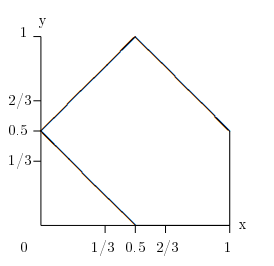
\includegraphics[width=6cm]{domain.png}
\end{figure}

\begin{enumerate}
    \item Найти погрешность аппроксимации разностной схемы на решении краевой задачи.
    \item Проверить, что функция $  \varphi(x,y)$ является точным решением краевой задачи.
    \item Для небольшого числа узлов сетки и двух вариантов нумерации внутренних узлов выписать в симметрическом виде матрицы $A$. Убедиться, что они являются симметричными и разреженными.
    \item Записать полученные матрицы в упакованном виде (по строкам).
    \item Найти максимальное и минимальное собственное значения матрицы $A$ для нескольких значений $m$ степенным методом.
    \item Используя собственные значения оператора $(Lv)_i=v_{i-1}-2v_i+v_{i+1},i=1,...,m-1, v_0=v_m=0$, найти собственные значения двумерного разностного оператора рассматриваемой задачи для $D=Q^2=[0,1]^2$. Сравнивать полученное значение $\lambda_{min}(h)$ с $\lambda_{min}$ для дифференциальной задачи. Получить асимптотическое разложение $\lambda_{min}(h)$ по $h$.
    \item Найти решение системы уравнений $Az=F$ методом установления и методом верхней релаксации.
    \item Для нескольких значений числа интервалов $m$ найти относительные погрешности разностного решения $	\Delta=<|U(x,y)-\varphi(x,y)|>/<|\varphi(x,y)|>.$
    
    Здесь $<|g(x,y)|>=\sum_{i,j}[(i,j)=\in D]|g(x_i,y_j)|.$
    \item Вывести на экран разностное решение $U(x,y)$ и погрешность $U(x,y)-\varphi(x,y)$.
    
\end{enumerate}

\section{Исследование данной схемы на точность и устойчивость.}

    \subsection{Погрешность аппроксимации.}
    Оценим погрешность аппроксимации данной задачи, для этого, Приблизим оператор Лапласа разностным оператором:
    \[
        \Lambda u = \Lambda_1 u + \Lambda_2 u = u_{x,x}+u_{y,y}
    \]
    Тогда с помощью разложения в ряд Тейлора получаем:
    \[
        \Lambda_1 u = {\dfrac{{\partial}^2 u}{\partial x^{2}}}+\dfrac{h^2}{12}{\dfrac{{\partial}^4 u}{\partial x^{4}}}+O(h^4)
    \]
    \[
         \Lambda_2 u = {\dfrac{{\partial}^2 u}{\partial y^{2}}}+\dfrac{h^2}{12}{\dfrac{{\partial}^4 u}{\partial y^{4}}}+O(h^4)
    \]
    Тогда
    \[
        \Lambda u - \Delta v = \dfrac{h^2}{12}{\dfrac{{\partial}^4 u}{\partial x^{4}}}+\dfrac{h^2}{12}{\dfrac{{\partial}^4 u}{\partial y^{4}}}+O(h^4)
    \]
    Отсюда следует, что
    \[
        \Lambda u - \Delta v = O(h^2)
    \]
    Таким образом, данный разностный оператор аппроксимирует оператор Лапласа со  вторым порядком аппроксимации на регулярном шаблоне "крест". 
    
\newpage

\section{Описание вычислительного метода. Алгоритм решения программы.}
\begin{itemize}
    \item Изобразим шаблон нашей схемы:
        \begin{figure}[h]
            \centering
            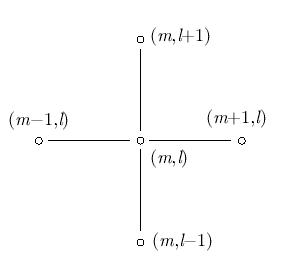
\includegraphics[width=6cm]{scheme.jpg}
        \end{figure}
    \item Наложим на нашу область равномерную сетку с шагом $h$     и пронумеруем узлы сетки следующим образом:
        \begin{figure}[h]
            \centering
            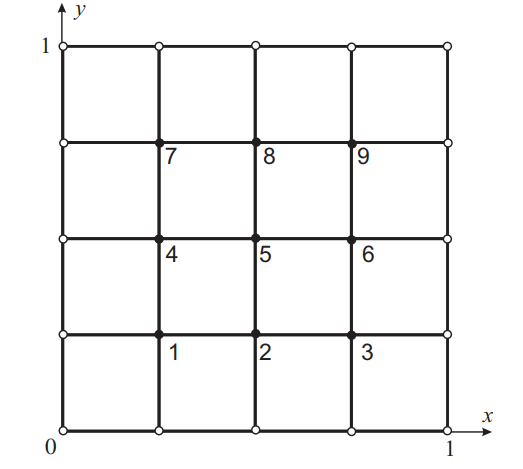
\includegraphics[width=6cm]{normal.png}
        \end{figure}
    \item С помощью отдельной функции, отделим точки, принадлежащие границе области D, точки, лежащие строго внутри области D и точки не принадлежащие области.  
    \item Для граничных точек сразу вычисляем значения искомой функции
    \item Для всех внутренних точек выполняем разностную схему и ищем их значения, как решение СЛАУ.На основе этого получаем матрицу.
    \item Записываем эту матрицу в упакованном виде
    \item Ищем у полученной матрицы max и min числа
    \item Решаем матрицу (СЛАУ) с помощью метода верхней релаксации и методом установления
    \item Заносим оставшиеся значения в матрицу решений и выводим полученный график
\end{itemize}
\newpage

\section{Код программы (на Pyton).}
	\begin{verbatim}
	
	\end{verbatim}
	
\section{Графический вывод (Тесты)}
При $h = 0.25$ 
\begin{figure}[h]
    \centering
    \includegraphics[width=14cm]{graph_u_1.png}
    \caption{график $u(x,y)$ при $h=0.25$}
\end{figure}
\\
Тогда максимальная ошибка и значения собственных чисел: 
\begin{figure}[h]
    \centering
    \includegraphics[width=6cm]{error_and_lambda_1.PNG}
\end{figure}
\\
При $h = 0.625$:
\begin{figure}[h]
    \centering
    \includegraphics[width=14cm]{graph_u_2.png}
    \caption{график $u(x,y)$ при $h=0.125$}
\end{figure}
\\
Тогда максимальная ошибка $0.01444$
\\

\begin{figure}[h]
    \centering
    \includegraphics[width=6cm]{error_and_lambda_2.png}
\end{figure}

\newpage

\section{Выводы.}

Таким образом мы исследовали задачу Дерихле в ограниченной области и изучили ход ее решения. Убедились в том, что при увеличении шага, погрешность решения уменьшается примерно в 2 раза.

Этот метод не очень прост в реализации: в нем участвуют сразу несколько дополнительных методов для поиска собственных чисел и решения системы линейных уравнений.Таким образом,данный метод можно разными способами модифицировать, что так же является плюсом метода.

\end{document}
